\documentclass[12pt, twoside]{article}
\usepackage[francais]{babel}
\usepackage[T1]{fontenc}
\usepackage[latin1]{inputenc}
\usepackage[left=7mm, right=1cm, top=1cm, bottom=7mm]{geometry}
\usepackage{float}
\usepackage{graphicx}
\usepackage{array}
\usepackage{multirow}
\usepackage{amsmath,amssymb,mathrsfs}
\usepackage{soul}
\usepackage{textcomp}
\usepackage{eurosym}
 \usepackage{variations}
\usepackage{tabvar}

\begin{document}


\section*{\center{Aide individualis�e: Triangles isom�triques}}

\subsection*{Rappels}

A l'aide de sch�ma, rappeler les 3 cas d'isom�tries de triangles.

\bigskip

\bigskip

\bigskip

\bigskip

\bigskip

\bigskip

\bigskip

\subsection*{Exercice 1}

Soit $ABCD$ un parall�logramme, $I$ le milieu de $[AB]$ et $J$ le milieu de
$[DC]$.


\textbf{On veut montrer que $ID=JB$.}



\subsubsection*{La recherche}

\begin{enumerate}
  \item Faire un sch�ma (pas trop petit) et coder la figure.
  \bigskip
  
  \bigskip
  
  \bigskip
  
  \bigskip
  
  \bigskip
  
  \bigskip
  
  \item Rep�rer les triangles qui semblent isom�triques (on ne demande pas de
  le justifier) et associer les sommets homologues.
  
  \bigskip
  
  \bigskip
  
  \bigskip
  
  
  \bigskip
  
  \bigskip
  
  \item Parmi les couples de triangles trouv�s, rep�rer ceux qui semblent
  inutile pour notre probl�me.
  
  
\end{enumerate}

\bigskip

\bigskip

\bigskip

\subsubsection*{La r�daction}

\begin{enumerate}
  \item Compl�ter:
  
  On se place dans les triangles $AID$ et \ldots \ldots
  
  $\ldots \ldots = BC$ car \ldots \ldots \ldots \ldots \ldots \ldots \ldots \ldots
  
  
  $AI=\ldots \ldots$ car \ldots \ldots \ldots \ldots \ldots \ldots \ldots \ldots
  
  $\widehat{DAI}=\widehat{JCA}$ car \ldots \ldots \ldots \ldots \ldots \ldots
  \ldots \ldots
  
   \item   \begin{tabular}{cc}
           
           \begin{minipage}{6cm}
  Coder le sch�ma suivant:
  \end{minipage}
  &
  \begin{minipage}{12cm}
  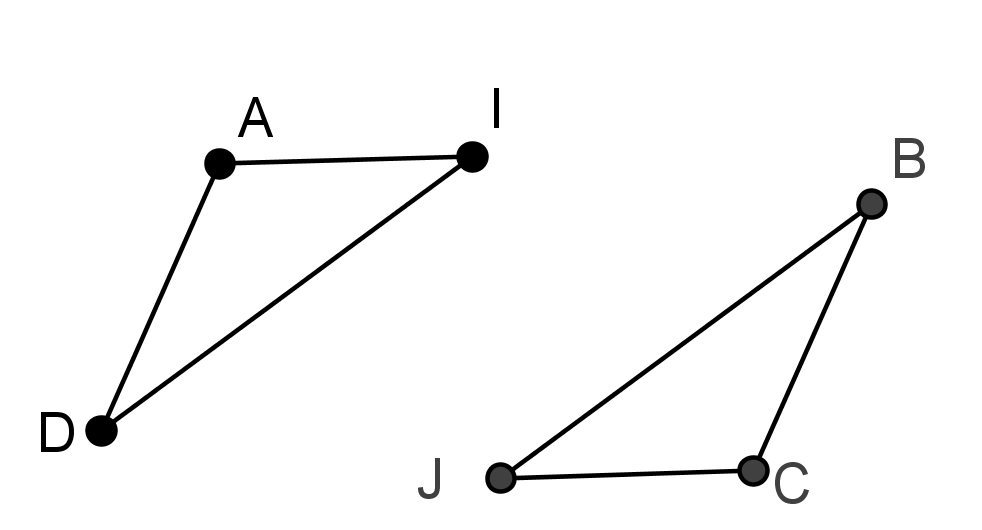
\includegraphics[width=6cm]{images/ex1.png}
  \end{minipage}
  \end{tabular}

\item Cela correspond-til � une des propri�t�s d'isom�tries des triangles? Si
oui, laquelle?

\bigskip

\bigskip

\item Conclure: Donc les triangles \ldots \ldots et \ldots \ldots sont \ldots
\ldots \ldots \ldots
\item Que peut-on en d�duire sur les angles et c�t�s homologues de ces deux
triangles? L'�crire.

\bigskip


\bigskip


\item Montrer que $ID=JB$.
\end{enumerate}


\subsection*{Exercice 2}

Soit $ABC$ un triangle quelquonque et $I$ le milieu de $[BC]$. 

$H$ est le point d'intersection de la droite perpendiculaire � $(AI)$ passant
par $B$ avec la droite $(AI)$.

$K$ est le point d'intersection de la droite perpendiculaire � $(AI)$ passant
par $C$ avec la droite $(AI)$.

\begin{center}
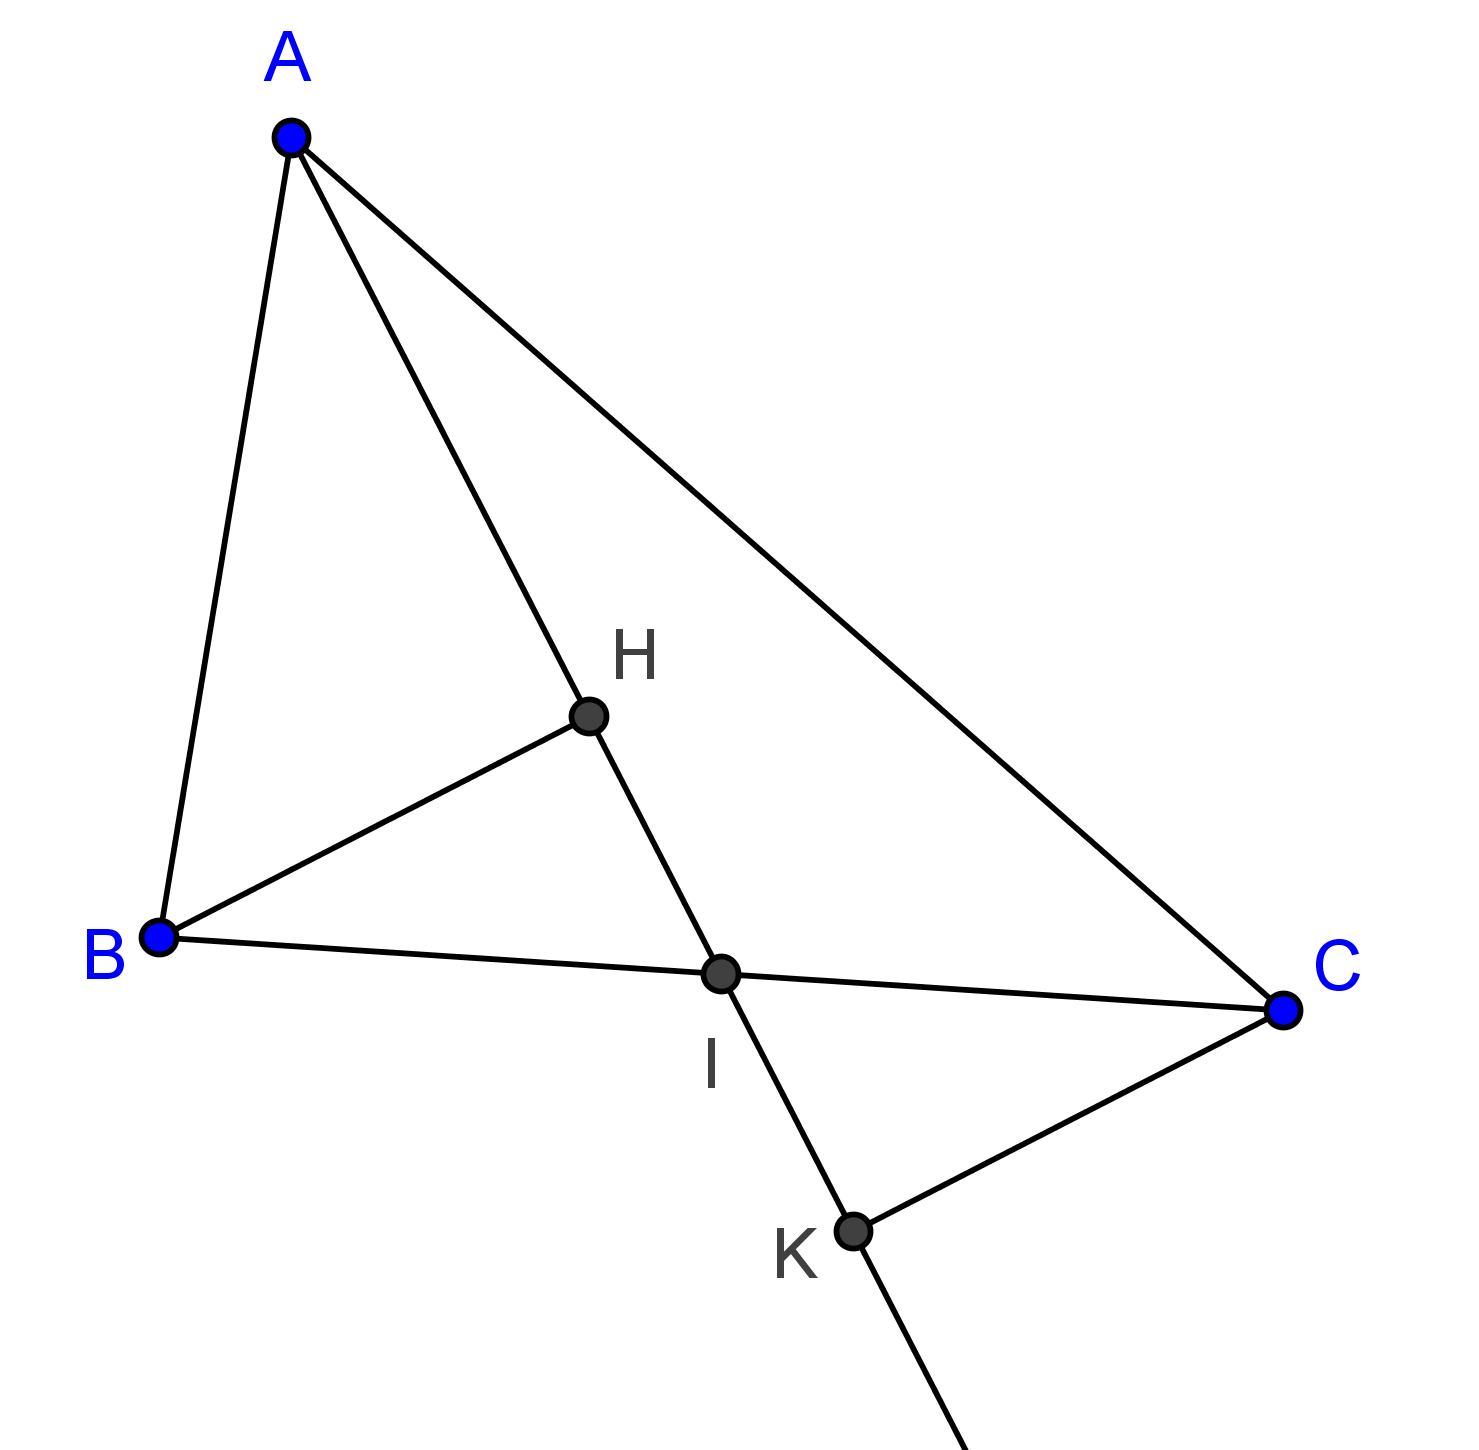
\includegraphics[width=6cm]{images/ex2.png}
\end{center} 

\begin{enumerate}
  \item Coder la figure.
  \item On cherche � montrer que les triangles $BHI$ et $CKI$ sont isom�triques.
  \begin{enumerate}
    \item Que peut-on dire des angles $\widehat{BHI}$ et $\widehat{CKI}$?
    
    \bigskip
    
    \item Que peut-on dire des longueurs $BI$ et $CI$? Justifier.
    
    \bigskip
    
    \item Sch�matiser les deux triangles concern�s, les coder puis associer les
    sommets homologues.
    
    \bigskip
    
    \bigskip
    
    \bigskip
    
    \bigskip
    
    \item Montrer que $\widehat{BIH}=\widehat{KIC}$ et reporter cette
    information sur votre sch�ma.
    
    \bigskip
    
    \bigskip
    
    \item Peut-on conclure? Pourquoi? 
    
    \bigskip
    
    \bigskip
    
    Conclusion: 
    
  \end{enumerate}
  
  \bigskip
  
  \item Montrer que $BH=CK$.
  \end{enumerate} 
\end{document}
